\section{results}


\begin{figure}
\centering
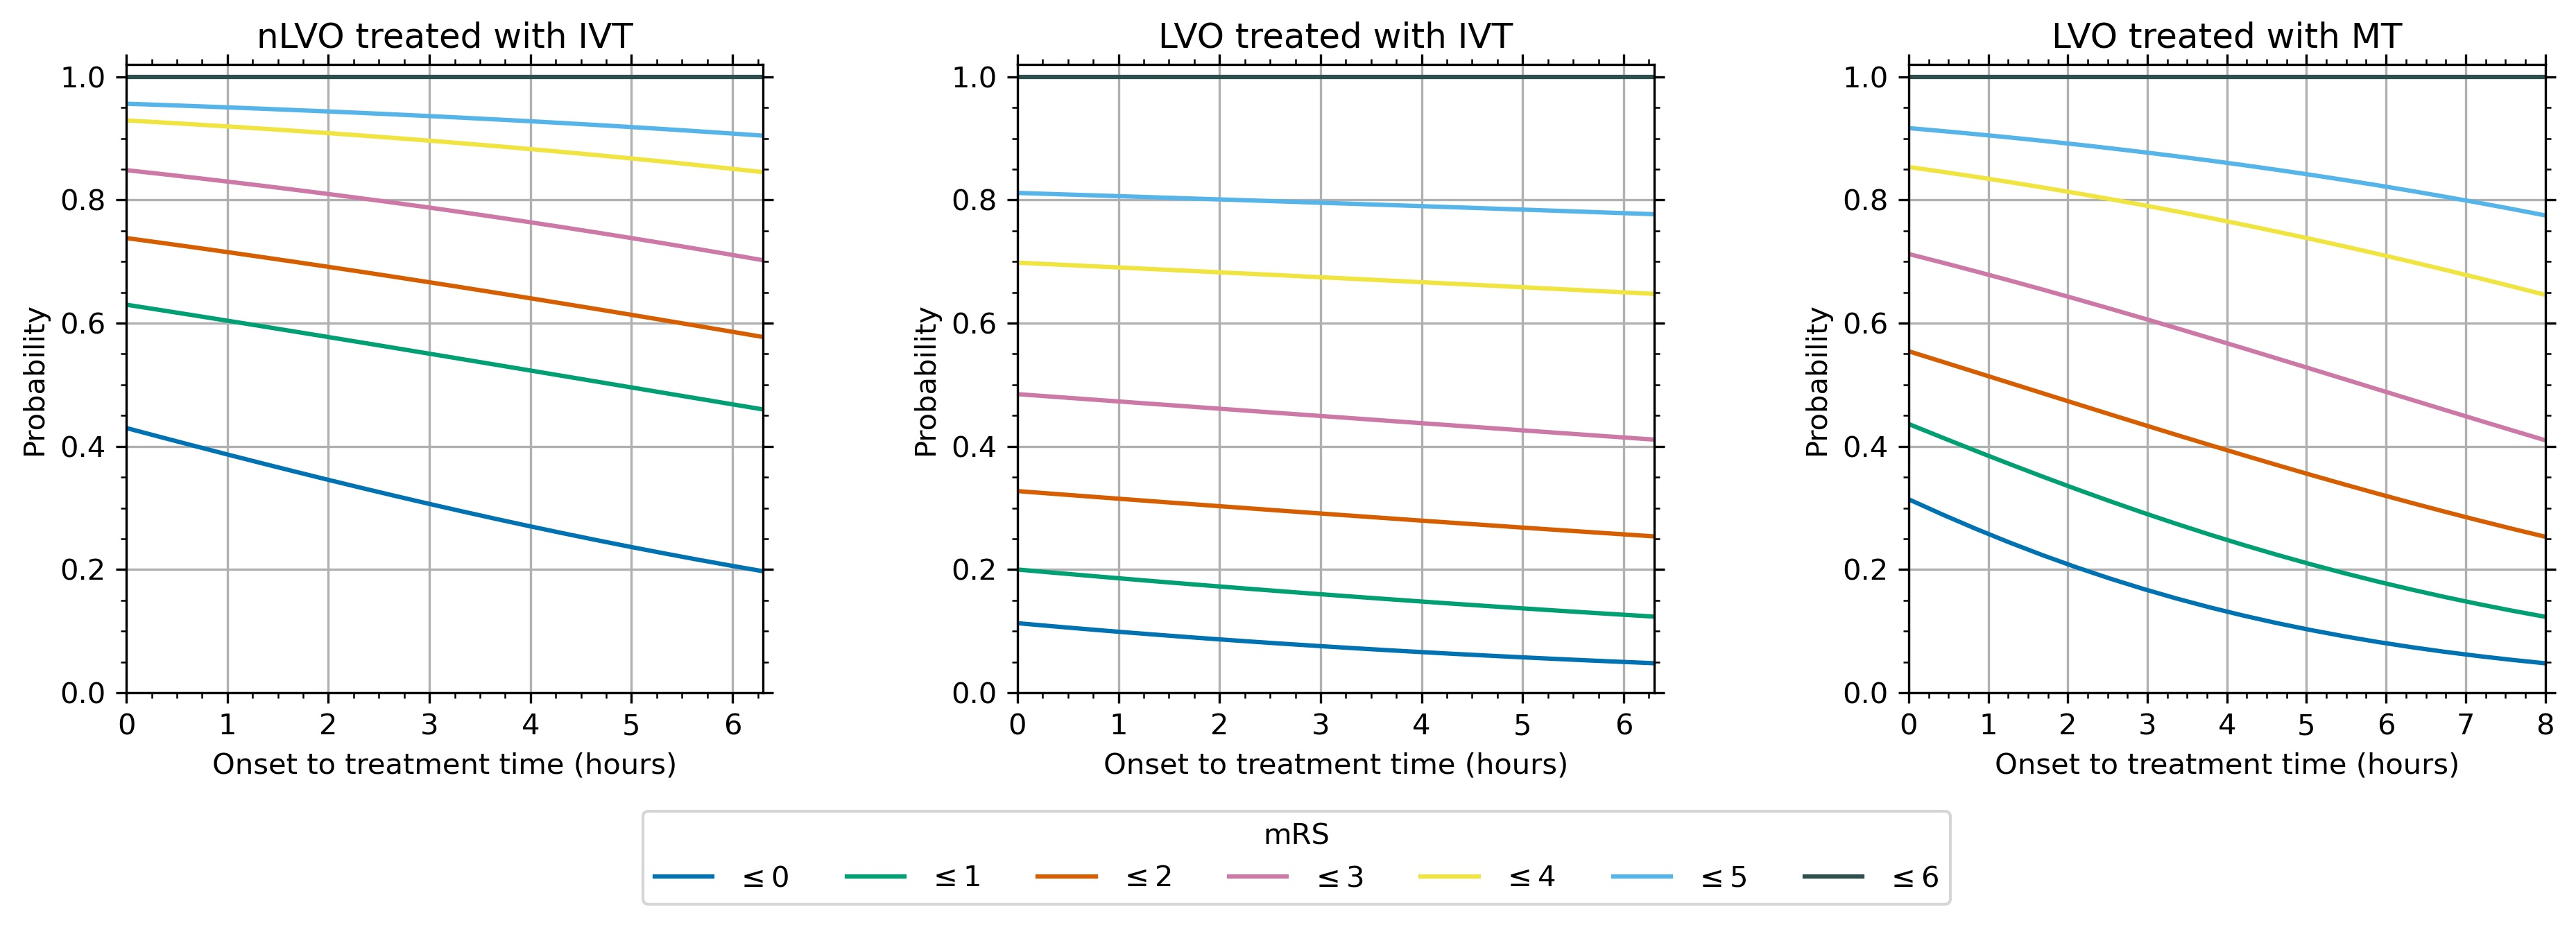
\includegraphics[width=1.0\textwidth]{./images/probs_with_time}
\caption{mRS probability distributions by time from onset to treatment. Left: nLVO treated with IVT. Middle: LVO treated with IVT. Right: LVO treated with MT.}
\label{fig:probs_with_time}
\end{figure}


\begin{figure}
\centering
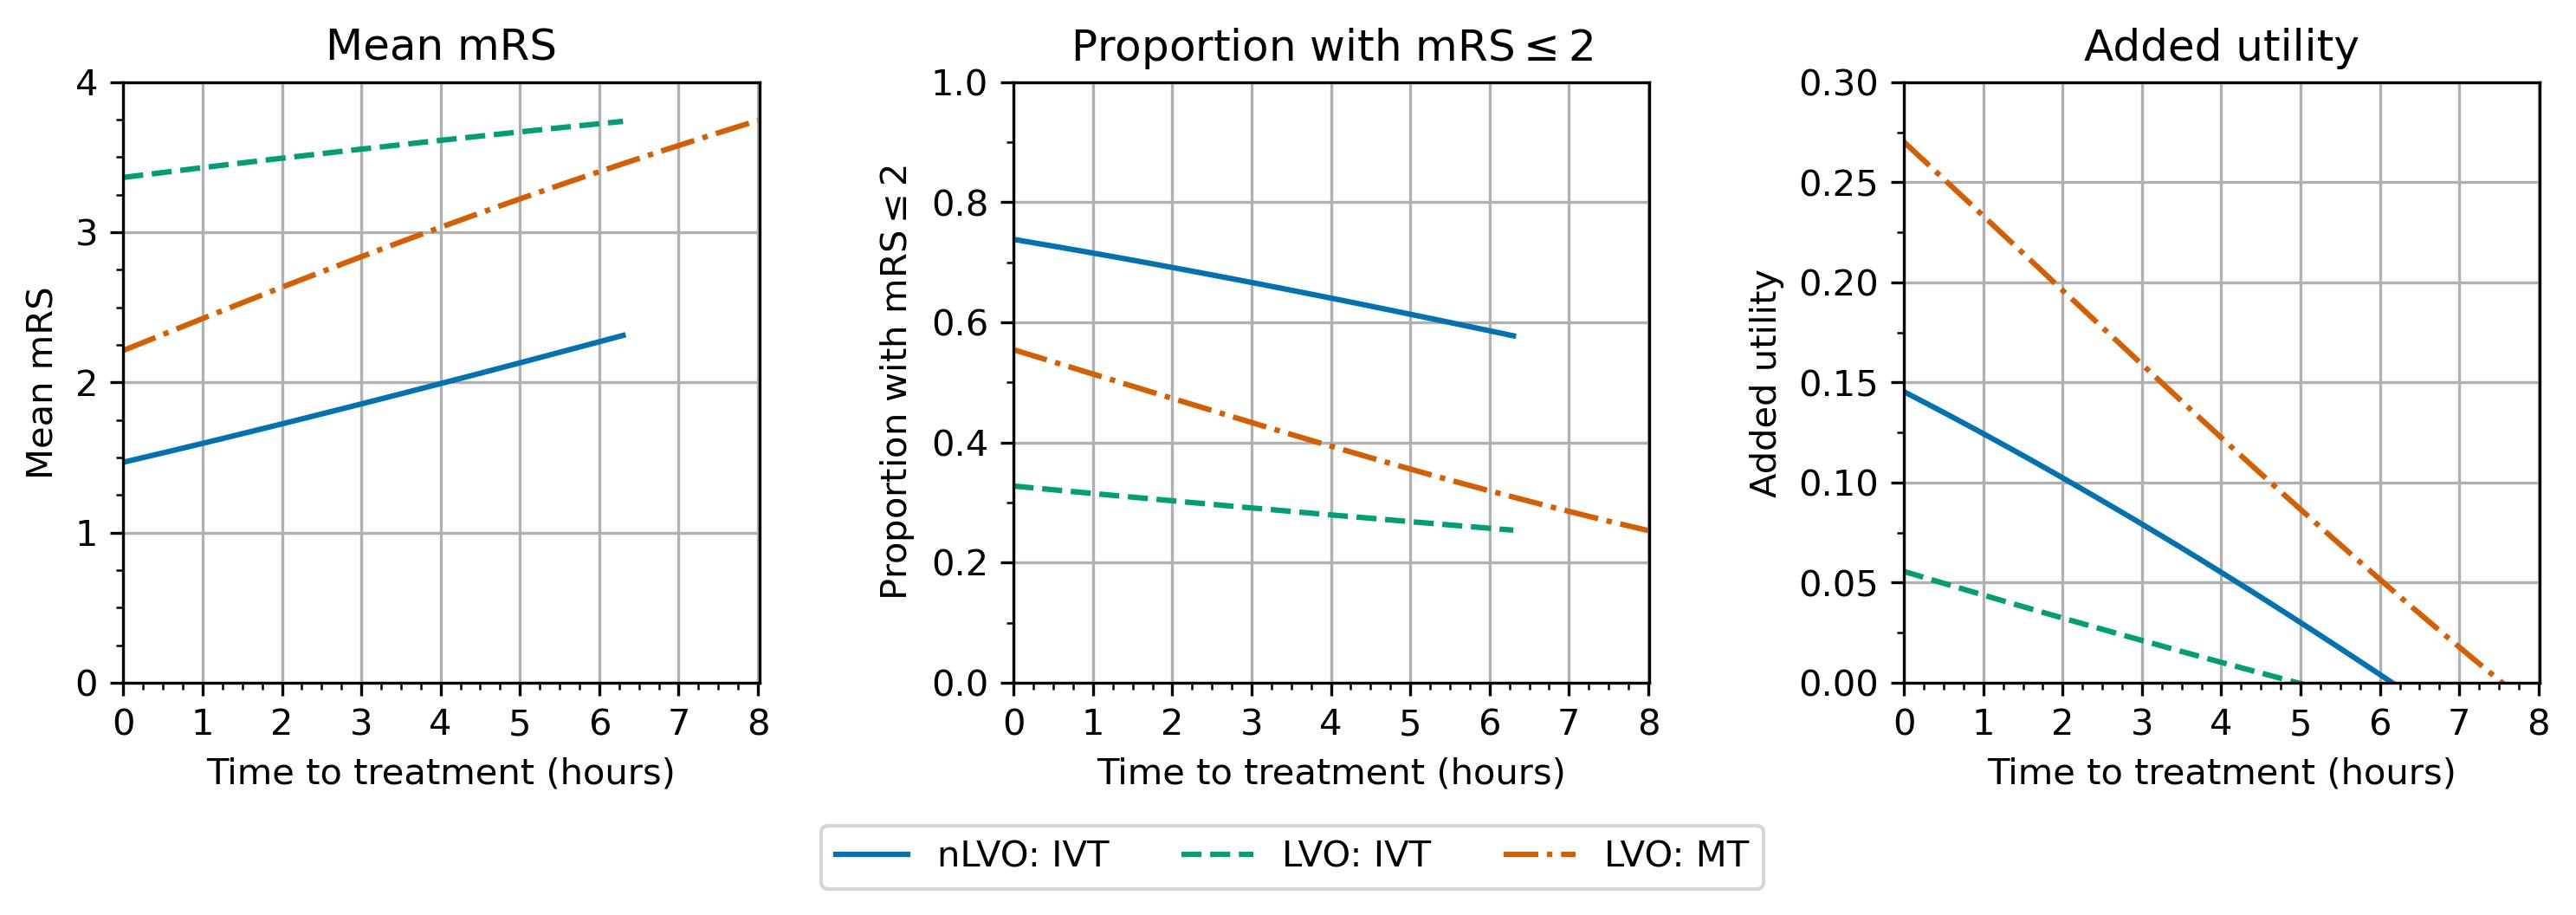
\includegraphics[width=1.0\textwidth]{./images/time_to_treatment}
\caption{Alternative outcome measures by by time from onset to treatment. Left: mean mRS. Middle: Proportion of patients with mRS 0-2. Right: Added utility.}
\label{fig:added_utility_six_in_one}
\end{figure}


\begin{figure}
\centering
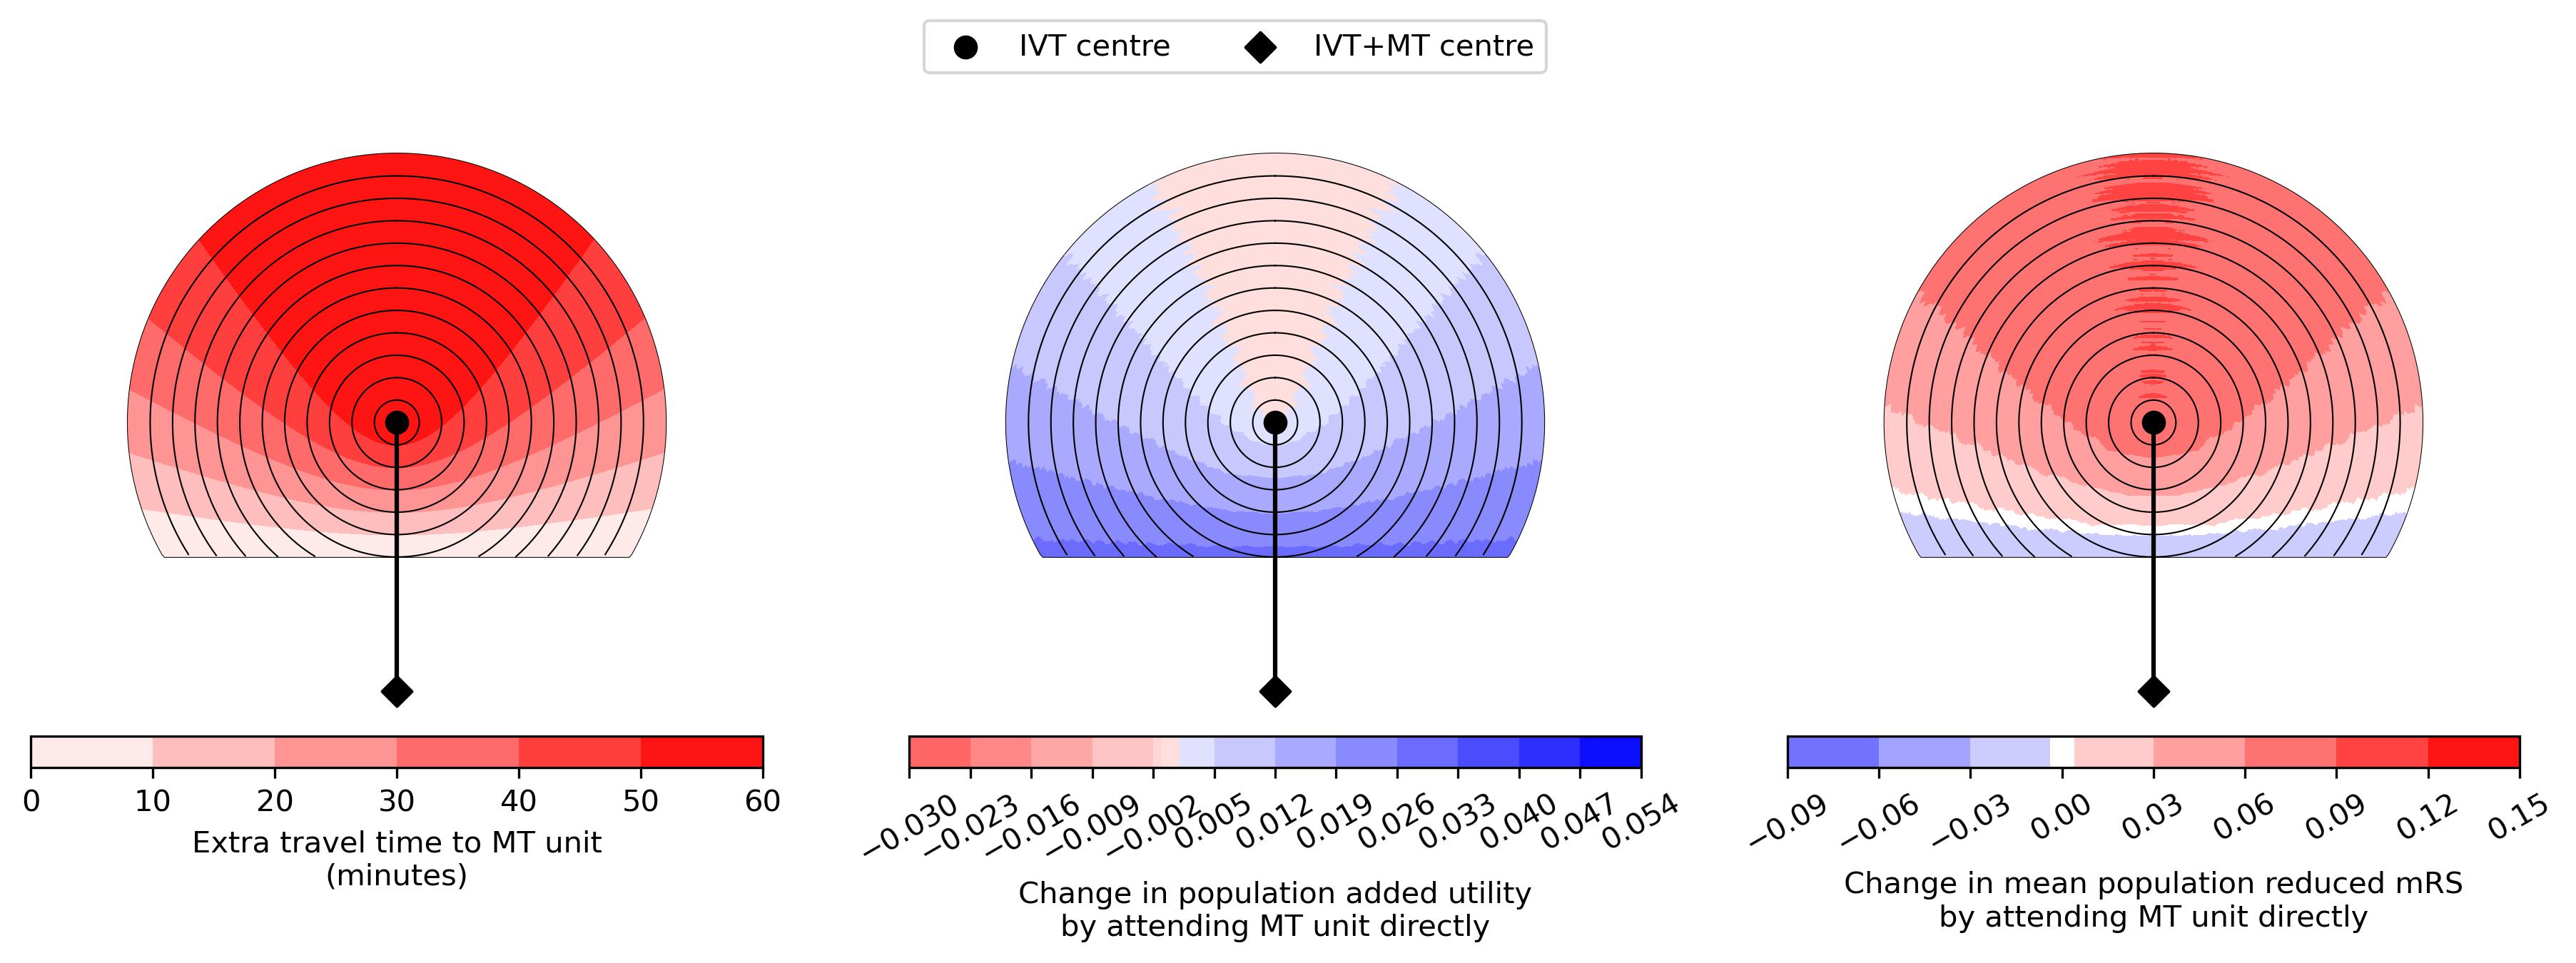
\includegraphics[width=1.0\textwidth]{./images/circle_plots_t-IVT-to-MT=60_t-onset-to-ambo=60}
\caption{The effect of bypassing an IVT-only unit in order to travel directly to a MT-capable unit that is 60 minutes away from the IVT-only unit. Results are for treatable patients (IVT and/or MT), with a mix of 35\% LVO and 65\% nLVO. An ambulance is assumed to arrive at the patient 60 minutes after stroke onset. Concentric circles represent 5 minutes travel time intervals from IVT-only unit. Left: Additional time required to attend the MT-capable unit  directly. Middle: Change in added utility by directly attending the MT-capable unit. Right: Change in population reduced average mRS by directly attending the MT-capable unit. Blue shades represent benefit, red shades represent disbenefit.}
\label{fig:added_utility_six_in_one}
\end{figure}

\begin{figure}
\centering
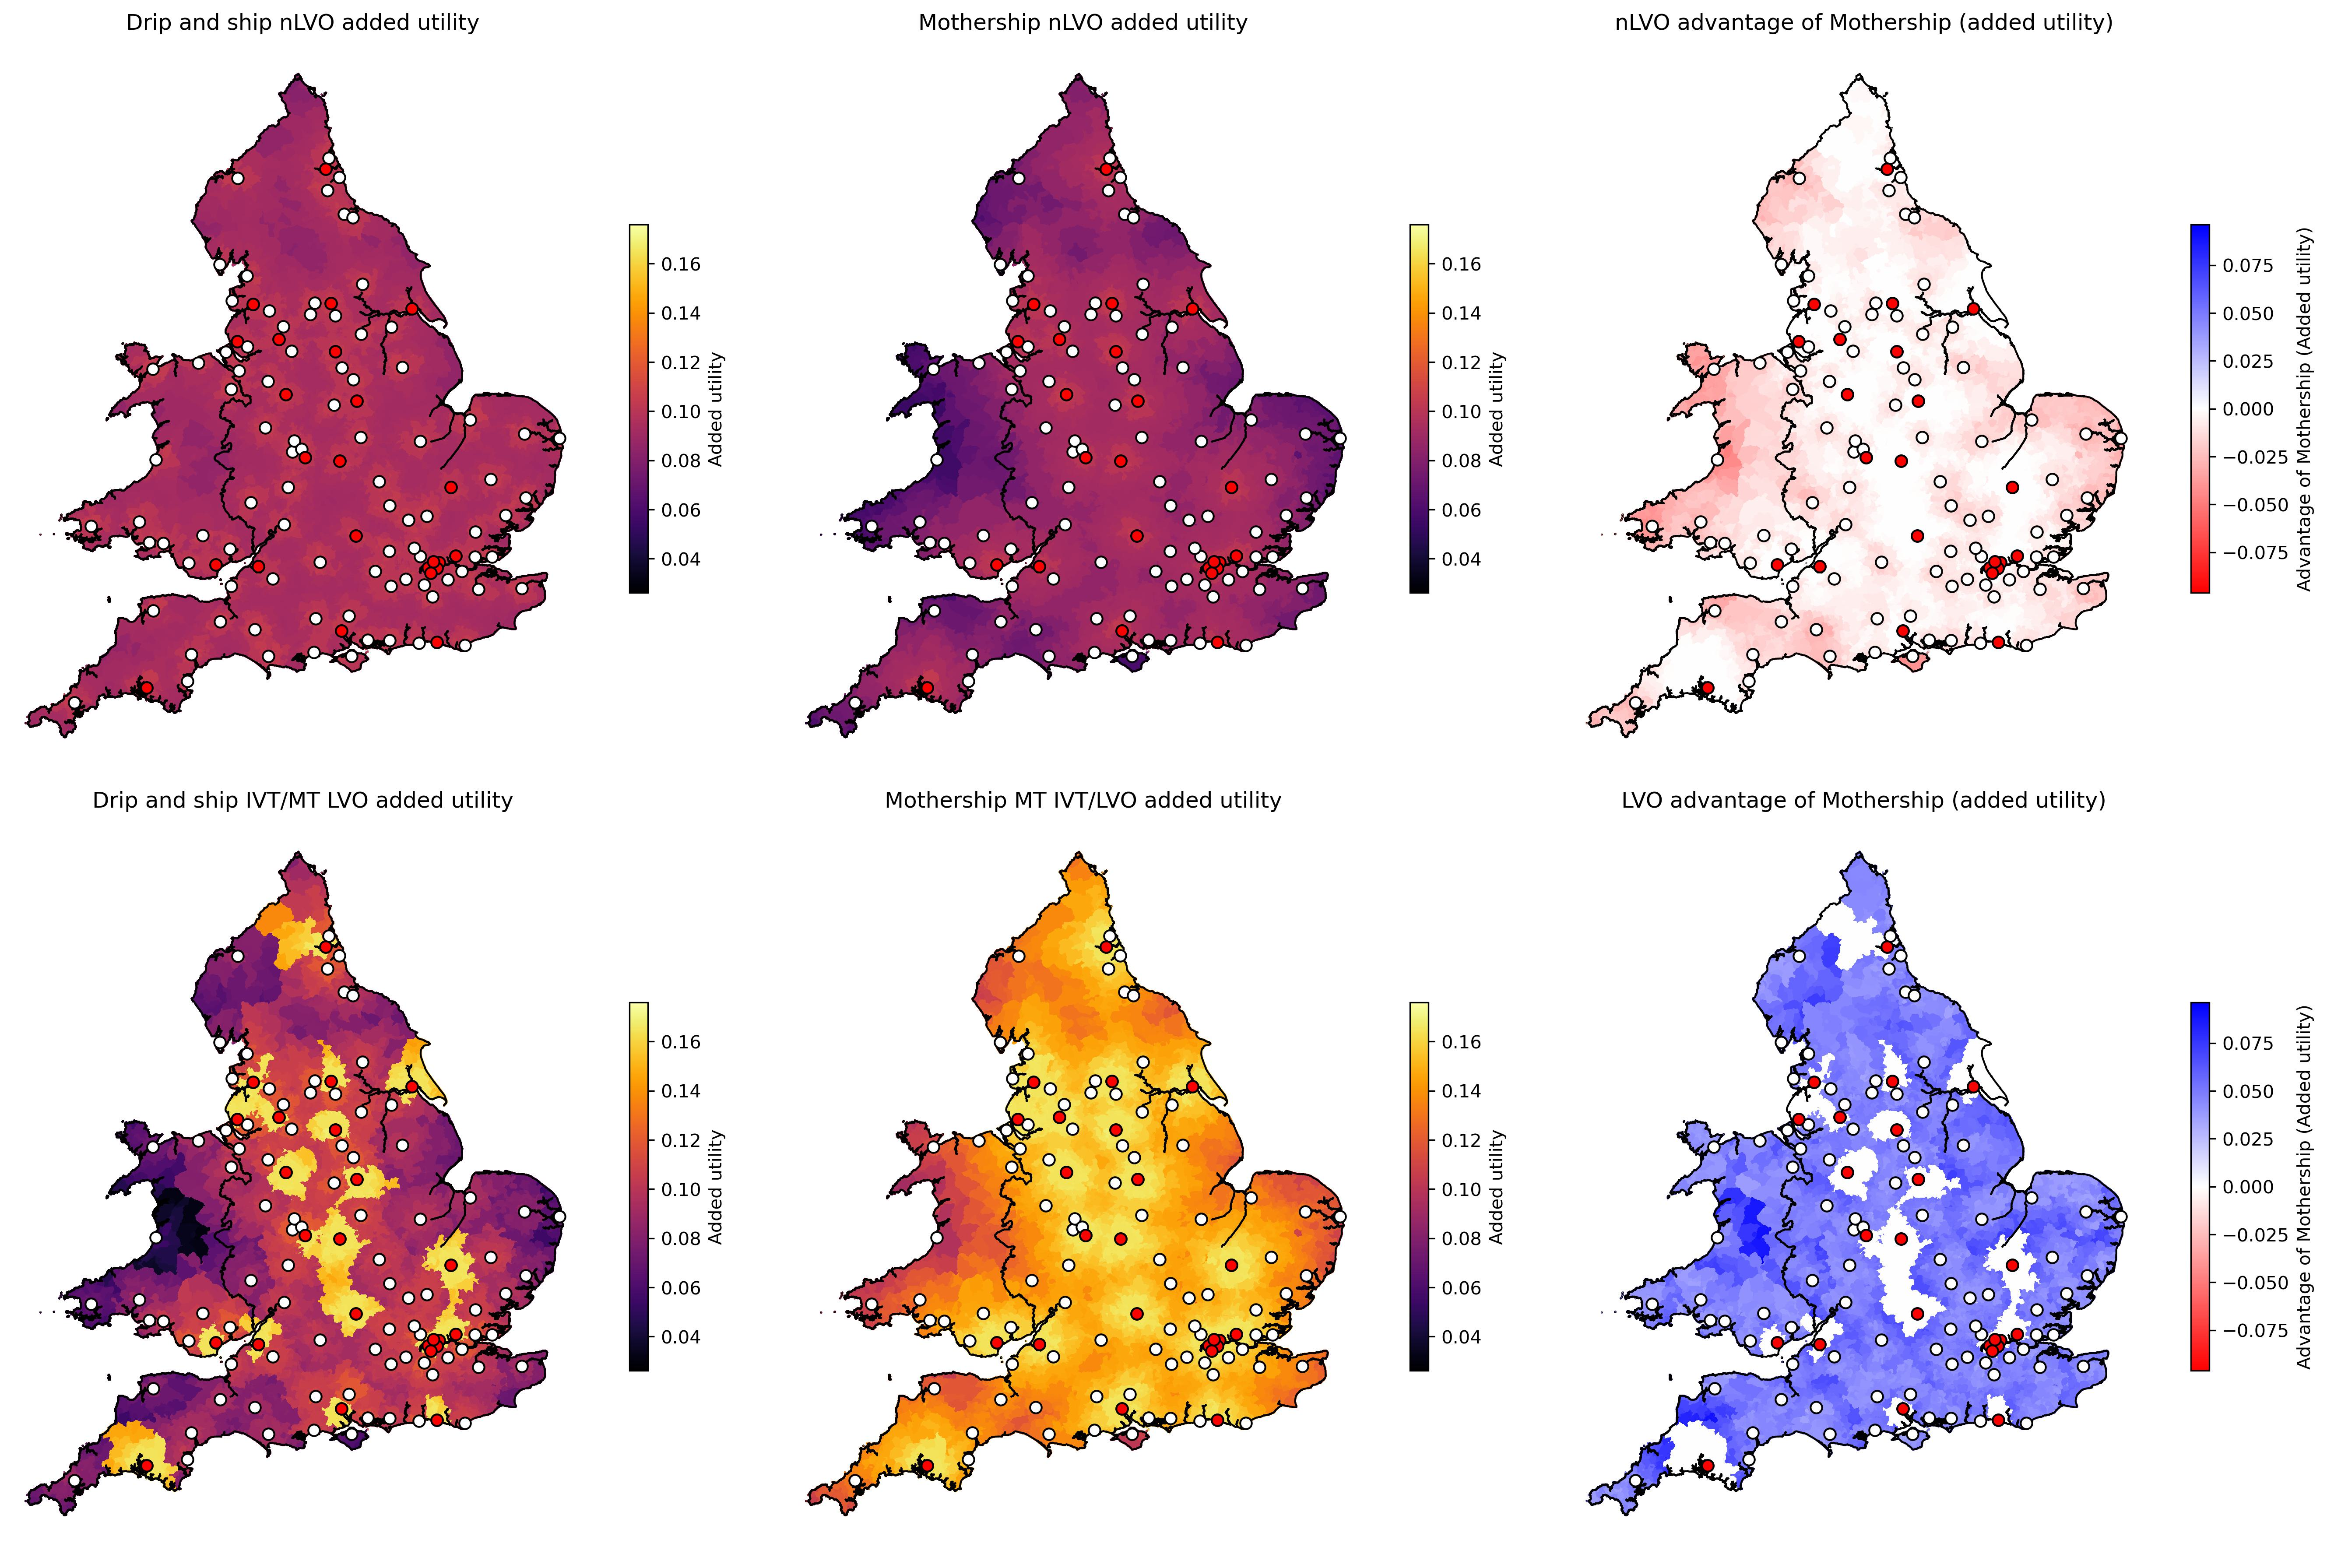
\includegraphics[width=1.0\textwidth]{./maps/added_utility_six_in_one}
\caption{Added utility from patients treated with IVT and/or MT. Top: nLVO treated with IVT. Bottom: LVO treated with IVT and/or MT. Left: Drip and ship. Middle: Mothership. Right: advantage of mothership over drip and ship. }
\label{fig:added_utility_six_in_one}
\end{figure}

\begin{figure}
\centering
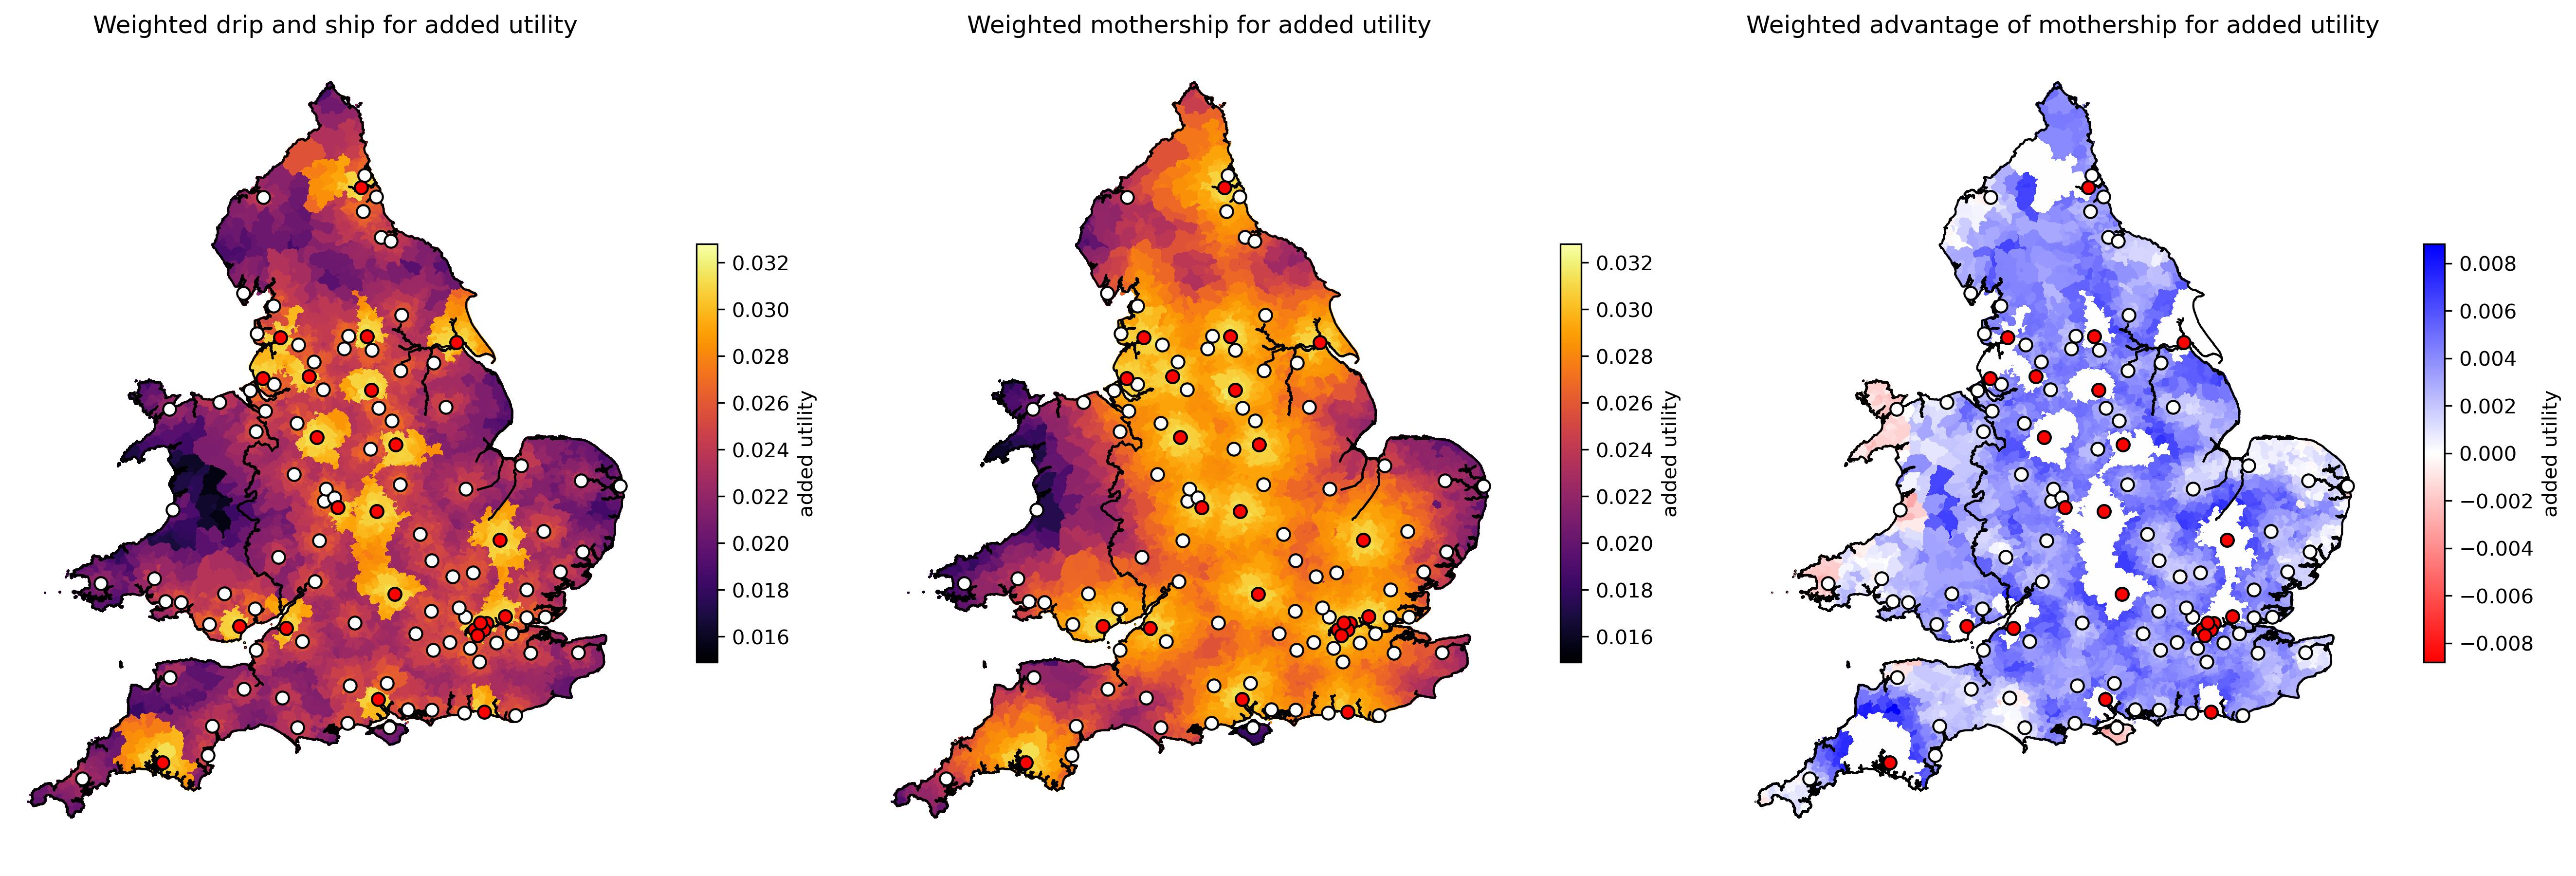
\includegraphics[width=1.0\textwidth]{./maps/added_utility_weighted_results}
\caption{Added utility }
\label{fig:added_utility_six_in_one}
\end{figure}